\documentclass[preprint,review,12pt,authoryear,times]{elsarticle}

\usepackage[section]{placeins}

\sloppy

\usepackage{stmaryrd,amssymb, linguex,setspace,dcolumn,multirow,longtable,hyperref,float}

\renewcommand{\firstrefdash}{}

\usepackage{lineno}

\newcommand{\tpa}{\textipa} %shorthand
\newcommand{\pp}{$\mid\mid$\hspace{0.2em}}
\newcommand{\ppp}{$\mid\mid\mid$\hspace{0.2em}}
\newcommand{\p}{$\mid$\hspace{0.2em}}
\newcommand{\g}{$\times$}

% adjust rows in tabular
\usepackage{array}

\journal{JPhon}

\begin{document}

\begin{frontmatter}


\title{The Effect of Focus Prominence on Phrasing: Supplementary materials}

\author{Michael Wagner\corref{cor1}}
\ead{chael@mcgill.ca}
\author{Michael McAuliffe\corref{cor2}}
\ead{michael.mcauliffe@mail.mcgill.ca}


\cortext[cor1]{Principal corresponding author}
\cortext[cor2]{Corresponding author}

\address{Department of Linguistics, McGill University \\ 1085 Doctor Penfield Avenue, Montr\'eal, Qu\'ebec, H3A 1A7\\Canada}

\end{frontmatter}


\tableofcontents

\newpage

\section{Additional plots}


\begin{figure*}[htb!]
	\begin{center}
		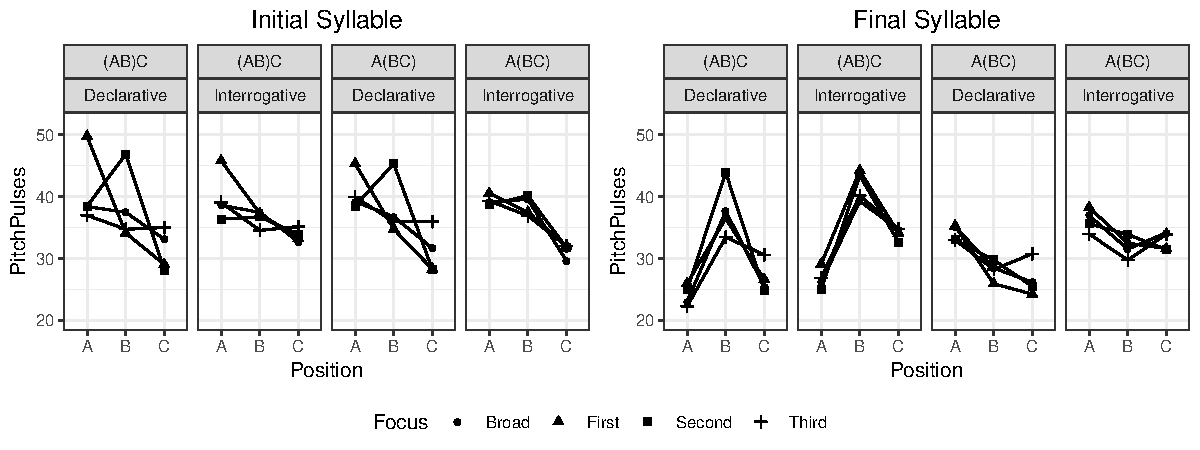
\includegraphics[width=5in]{Figures/PitchPulses.pdf}
		\caption{Number of pitch pulses of initial and final syllable for each target word}
		\label{figurePitchPulses}
	\end{center}
\end{figure*}

\begin{figure*}[ht!]
	\begin{center}
	{\footnotesize
		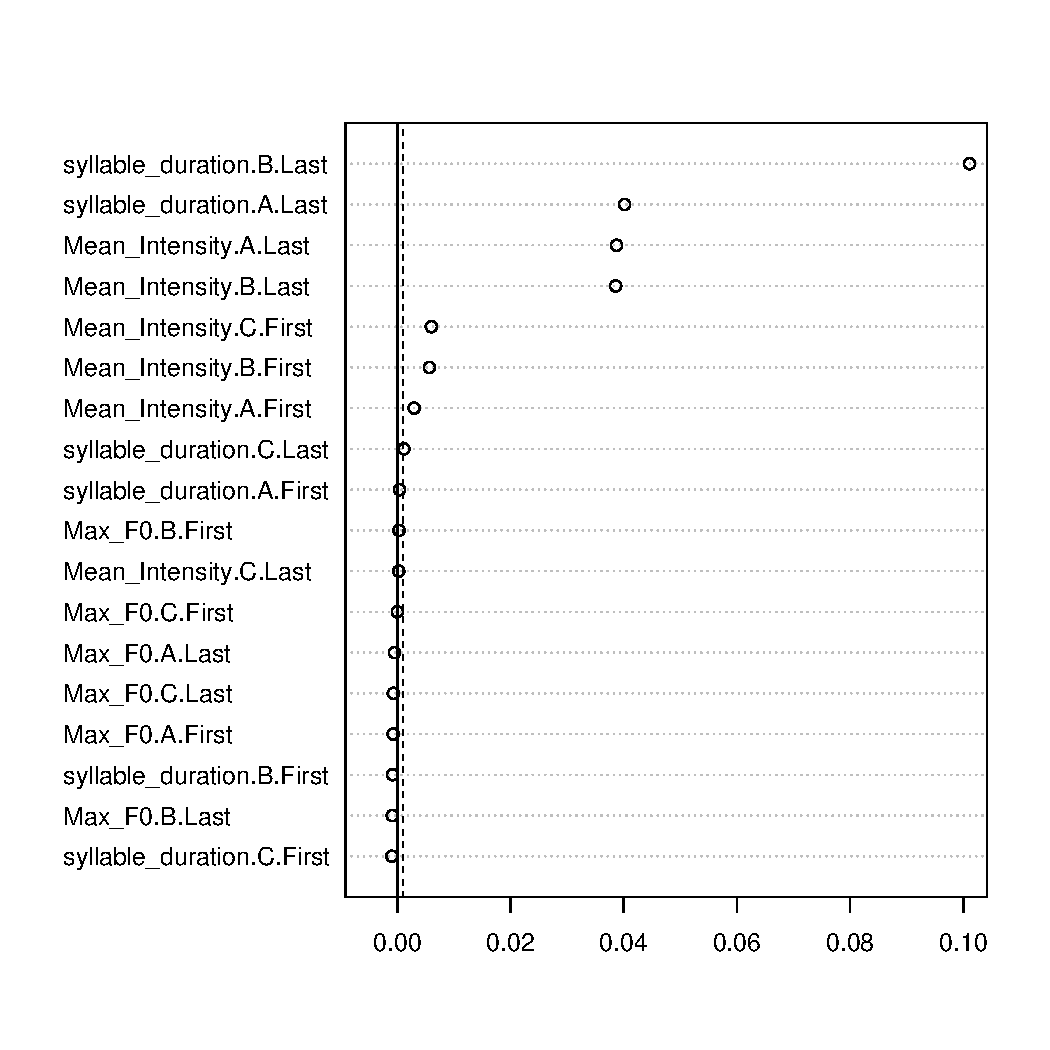
\includegraphics[width=2.8in]{Figures/phrasingFirstCVarimp.pdf}	
		}
		\caption{Importance of variables in random forest classification of Constituency for the case of broad focus (left) and first focus (right) respectively}
		\label{focusForestFirstC}
	\end{center}
\end{figure*}


\begin{figure*}[htb!]
	\begin{center}
		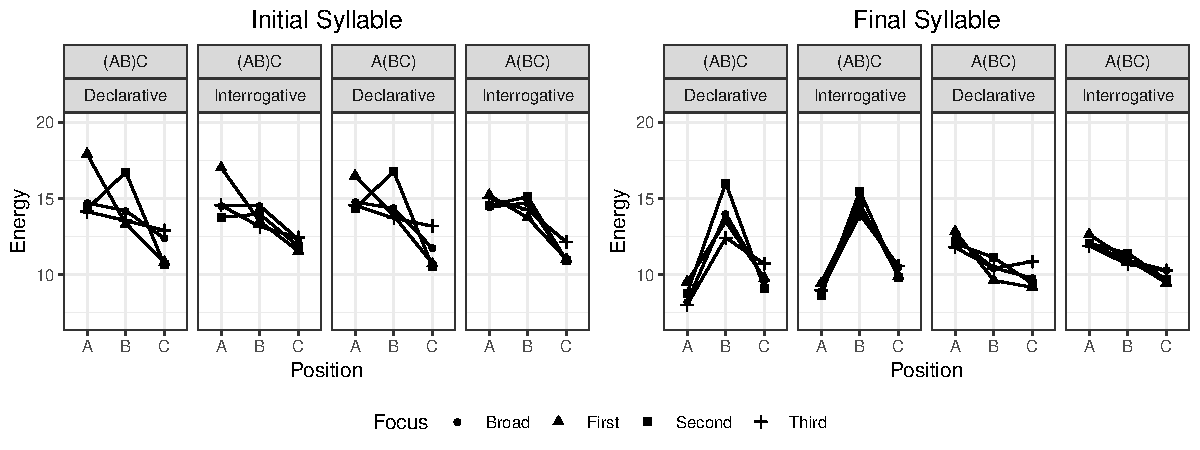
\includegraphics[width=5in]{Figures/Energy.pdf}
		\caption{Energy of initial and final syllable for each target word}
		\label{figureEnergy}
	\end{center}
\end{figure*}


\newpage
\section{Regression models for word A and word C}


\begin{table}[h!]
\begin{center}
\begin{footnotesize}
\begin{tabular}{l D{)}{)}{11)3} D{)}{)}{11)3} }
\hline
 & \multicolumn{1}{c}{Initial} & \multicolumn{1}{c}{Final} \\
\hline
(Intercept)                                 & 0.22 \; (0.02)^{***}  & 0.16 \; (0.02)^{**}  \\
Broad.vs.Narrow                             & 0.01 \; (0.01)        & 0.00 \; (0.00)       \\
First.vs.Late                               & -0.03 \; (0.01)^{***} & -0.01 \; (0.00)^{**} \\
Second.vs.Third                             & 0.00 \; (0.01)        & -0.00 \; (0.00)      \\
Decl.vs.Inter                               & 0.00 \; (0.00)        & 0.00 \; (0.00)       \\
Left.vs.Right                               & -0.00 \; (0.00)       & 0.05 \; (0.01)^{***} \\
Broad.vs.Narrow:Decl.vs.Inter               & -0.00 \; (0.01)       & -0.00 \; (0.01)      \\
First.vs.Late:Decl.vs.Inter                 & 0.01 \; (0.01)        & 0.01 \; (0.01)       \\
Second.vs.Third:Decl.vs.Inter               & 0.00 \; (0.01)        & 0.00 \; (0.01)       \\
Broad.vs.Narrow:Left.vs.Right               & -0.00 \; (0.01)       & -0.01 \; (0.01)      \\
First.vs.Late:Left.vs.Right                 & 0.03 \; (0.01)^{***}  & 0.00 \; (0.01)       \\
Second.vs.Third:Left.vs.Right               & -0.00 \; (0.01)       & 0.00 \; (0.01)       \\
Decl.vs.Inter:Left.vs.Right                 & 0.01 \; (0.01)        & -0.01 \; (0.01)      \\
Broad.vs.Narrow:Decl.vs.Inter:Left.vs.Right & 0.01 \; (0.01)        & 0.02 \; (0.01)       \\
First.vs.Late:Decl.vs.Inter:Left.vs.Right   & 0.00 \; (0.01)        & -0.00 \; (0.01)      \\
Second.vs.Third:Decl.vs.Inter:Left.vs.Right & -0.01 \; (0.02)       & -0.03 \; (0.02)^{*}  \\
\hline
\multicolumn{3}{l}{\tiny{$^{***}p<0.001$, $^{**}p<0.01$, $^*p<0.05$}}
\end{tabular}
\end{footnotesize}
\caption{Mixed Effects Regression Models for the duration of word A (estimate in ms, SE in parentheses).}
\label{modelDurationA}
\end{center}
\end{table}



\begin{table}[h!]
\begin{center}
\begin{footnotesize}
\begin{tabular}{l D{)}{)}{11)3} D{)}{)}{11)2} }
\hline
 & \multicolumn{1}{c}{Initial} & \multicolumn{1}{c}{Final} \\
\hline
(Intercept)                                 & 0.18 \; (0.03)^{**}   & 0.16 \; (0.03)^{**} \\
Broad.vs.Narrow                             & -0.00 \; (0.00)       & -0.00 \; (0.00)     \\
First.vs.Late                               & 0.01 \; (0.01)        & 0.01 \; (0.00)      \\
Second.vs.Third                             & 0.02 \; (0.01)^{*}    & 0.01 \; (0.01)      \\
Decl.vs.Inter                               & 0.00 \; (0.00)        & -0.00 \; (0.00)     \\
Left.vs.Right                               & -0.01 \; (0.00)       & -0.00 \; (0.00)     \\
Broad.vs.Narrow:Decl.vs.Inter               & 0.00 \; (0.00)        & -0.01 \; (0.00)^{*} \\
First.vs.Late:Decl.vs.Inter                 & -0.01 \; (0.00)       & 0.00 \; (0.00)      \\
Second.vs.Third:Decl.vs.Inter               & -0.02 \; (0.01)^{***} & -0.01 \; (0.01)^{*} \\
Broad.vs.Narrow:Left.vs.Right               & 0.01 \; (0.00)        & -0.01 \; (0.00)     \\
First.vs.Late:Left.vs.Right                 & 0.01 \; (0.00)        & 0.01 \; (0.00)^{*}  \\
Second.vs.Third:Left.vs.Right               & 0.00 \; (0.01)        & -0.01 \; (0.01)     \\
Decl.vs.Inter:Left.vs.Right                 & -0.01 \; (0.00)^{*}   & -0.00 \; (0.00)     \\
Broad.vs.Narrow:Decl.vs.Inter:Left.vs.Right & 0.00 \; (0.01)        & -0.00 \; (0.01)     \\
First.vs.Late:Decl.vs.Inter:Left.vs.Right   & 0.00 \; (0.01)        & -0.01 \; (0.01)     \\
Second.vs.Third:Decl.vs.Inter:Left.vs.Right & 0.00 \; (0.01)        & -0.01 \; (0.01)     \\
\hline
\multicolumn{3}{l}{\tiny{$^{***}p<0.001$, $^{**}p<0.01$, $^*p<0.05$}}
\end{tabular}
\end{footnotesize}
\caption{Mixed Effects Regression Models for the duration of word C (estimate in sec, SE in parentheses).}
\label{modelDurationC}
\end{center}
\end{table}



\begin{table}[h!]
\begin{center}
\begin{footnotesize}
\begin{tabular}{l D{)}{)}{11)3} D{)}{)}{11)3} }
\hline
 & \multicolumn{1}{c}{Initial} & \multicolumn{1}{c}{Final} \\
\hline
(Intercept)                                 & 62.54 \; (1.22)^{***} & 58.78 \; (1.04)^{***} \\
Broad.vs.Narrow                             & 0.13 \; (0.19)        & -0.55 \; (0.40)       \\
First.vs.Late                               & 0.10 \; (0.20)        & 0.53 \; (0.30)        \\
Second.vs.Third                             & 0.01 \; (0.19)        & 0.35 \; (0.26)        \\
Decl.vs.Inter                               & -0.44 \; (0.34)       & 0.64 \; (0.36)        \\
Left.vs.Right                               & 0.49 \; (0.21)        & -2.94 \; (0.78)^{*}   \\
Broad.vs.Narrow:Decl.vs.Inter               & -0.18 \; (0.31)       & -0.21 \; (0.42)       \\
First.vs.Late:Decl.vs.Inter                 & 0.69 \; (0.34)^{*}    & -1.10 \; (0.46)^{*}   \\
Second.vs.Third:Decl.vs.Inter               & -0.22 \; (0.39)       & -0.38 \; (0.52)       \\
Broad.vs.Narrow:Left.vs.Right               & -0.44 \; (0.31)       & 0.51 \; (0.42)        \\
First.vs.Late:Left.vs.Right                 & -0.76 \; (0.34)^{*}   & 0.12 \; (0.46)        \\
Second.vs.Third:Left.vs.Right               & -0.18 \; (0.38)       & -0.69 \; (0.52)       \\
Decl.vs.Inter:Left.vs.Right                 & -0.31 \; (0.27)       & 0.32 \; (0.37)        \\
Broad.vs.Narrow:Decl.vs.Inter:Left.vs.Right & -0.28 \; (0.62)       & -0.63 \; (0.84)       \\
First.vs.Late:Decl.vs.Inter:Left.vs.Right   & 0.59 \; (0.68)        & -0.42 \; (0.92)       \\
Second.vs.Third:Decl.vs.Inter:Left.vs.Right & 0.79 \; (0.77)        & 2.19 \; (1.05)^{*}    \\
\hline
\multicolumn{3}{l}{\tiny{$^{***}p<0.001$, $^{**}p<0.01$, $^*p<0.05$}}
\end{tabular}
\end{footnotesize}
\caption{Mixed Effects Regression Models for the mean intensity of word A (estimate in dB, SE in parentheses).}
\label{modelIntensityA}
\end{center}
\end{table}



\begin{table}[h!]
\begin{center}
\begin{footnotesize}
\begin{tabular}{l D{)}{)}{11)3} D{)}{)}{11)3} }
\hline
 & \multicolumn{1}{c}{Initial} & \multicolumn{1}{c}{Final} \\
\hline
(Intercept)                                 & 60.78 \; (1.30)^{***} & 57.72 \; (1.40)^{***} \\
Broad.vs.Narrow                             & -0.53 \; (0.19)       & -0.51 \; (0.31)       \\
First.vs.Late                               & 0.10 \; (0.21)        & 0.02 \; (0.19)        \\
Second.vs.Third                             & 1.07 \; (0.24)^{*}    & 0.68 \; (0.23)        \\
Decl.vs.Inter                               & 0.03 \; (0.29)        & 3.22 \; (0.48)^{***}  \\
Left.vs.Right                               & -0.36 \; (0.20)       & -0.00 \; (0.18)       \\
Broad.vs.Narrow:Decl.vs.Inter               & 1.24 \; (0.35)^{***}  & 1.04 \; (0.36)^{**}   \\
First.vs.Late:Decl.vs.Inter                 & -1.05 \; (0.38)^{**}  & -0.17 \; (0.39)       \\
Second.vs.Third:Decl.vs.Inter               & -1.76 \; (0.43)^{***} & -0.58 \; (0.44)       \\
Broad.vs.Narrow:Left.vs.Right               & 0.06 \; (0.35)        & 0.20 \; (0.36)        \\
First.vs.Late:Left.vs.Right                 & 0.32 \; (0.38)        & -0.46 \; (0.39)       \\
Second.vs.Third:Left.vs.Right               & 0.04 \; (0.43)        & -0.06 \; (0.44)       \\
Decl.vs.Inter:Left.vs.Right                 & 0.16 \; (0.30)        & -0.20 \; (0.31)       \\
Broad.vs.Narrow:Decl.vs.Inter:Left.vs.Right & -0.89 \; (0.69)       & -0.06 \; (0.71)       \\
First.vs.Late:Decl.vs.Inter:Left.vs.Right   & -0.63 \; (0.76)       & -0.09 \; (0.78)       \\
Second.vs.Third:Decl.vs.Inter:Left.vs.Right & -1.53 \; (0.86)       & 0.13 \; (0.88)        \\
\hline
\multicolumn{3}{l}{\tiny{$^{***}p<0.001$, $^{**}p<0.01$, $^*p<0.05$}}
\end{tabular}
\end{footnotesize}
\caption{Mixed Effects Regression Models for the mean intensity of word C (estimate in dB, SE in parentheses).}
\label{modelIntensityC}
\end{center}
\end{table}



\begin{table}[h!]
\begin{center}
\begin{footnotesize}
\begin{tabular}{l D{)}{)}{12)3} D{)}{)}{12)3} }
\hline
 & \multicolumn{1}{c}{Initial} & \multicolumn{1}{c}{Final} \\
\hline
(Intercept)                                 & 199.66 \; (8.23)^{***} & 197.04 \; (9.02)^{***} \\
Broad.vs.Narrow                             & 2.55 \; (3.00)         & -4.00 \; (1.85)^{*}    \\
First.vs.Late                               & -12.99 \; (5.01)^{*}   & -5.24 \; (2.74)        \\
Second.vs.Third                             & 3.40 \; (1.79)         & 3.69 \; (2.08)         \\
Decl.vs.Inter                               & -5.16 \; (2.79)        & 12.98 \; (3.71)^{**}   \\
Left.vs.Right                               & 2.68 \; (2.34)         & 3.17 \; (2.66)         \\
Broad.vs.Narrow:Decl.vs.Inter               & -5.18 \; (2.88)        & 0.43 \; (3.37)         \\
First.vs.Late:Decl.vs.Inter                 & 8.87 \; (3.17)^{**}    & -10.72 \; (3.69)^{**}  \\
Second.vs.Third:Decl.vs.Inter               & -0.83 \; (3.59)        & 4.21 \; (4.16)         \\
Broad.vs.Narrow:Left.vs.Right               & -0.21 \; (2.89)        & -3.14 \; (3.37)        \\
First.vs.Late:Left.vs.Right                 & 2.78 \; (3.17)         & -6.23 \; (3.69)        \\
Second.vs.Third:Left.vs.Right               & 0.11 \; (3.57)         & -3.67 \; (4.16)        \\
Decl.vs.Inter:Left.vs.Right                 & -0.24 \; (2.55)        & 0.82 \; (2.97)         \\
Broad.vs.Narrow:Decl.vs.Inter:Left.vs.Right & 1.85 \; (5.77)         & -3.96 \; (6.73)        \\
First.vs.Late:Decl.vs.Inter:Left.vs.Right   & -3.25 \; (6.34)        & 1.54 \; (7.38)         \\
Second.vs.Third:Decl.vs.Inter:Left.vs.Right & -7.04 \; (7.18)        & -7.62 \; (8.33)        \\
\hline
\multicolumn{3}{l}{\tiny{$^{***}p<0.001$, $^{**}p<0.01$, $^*p<0.05$}}
\end{tabular}
\end{footnotesize}
\caption{Mixed Effects Regression Models for the Max F$_0$ of word A (estimate in Hz, SE in parentheses).}
\label{modelPitchA}
\end{center}
\end{table}



\begin{table}[h!]
\begin{center}
\begin{footnotesize}
\begin{tabular}{l D{)}{)}{12)3} D{)}{)}{12)3} }
\hline
 & \multicolumn{1}{c}{Initial} & \multicolumn{1}{c}{Final} \\
\hline
(Intercept)                                 & 190.54 \; (7.65)^{***} & 197.40 \; (8.84)^{***} \\
Broad.vs.Narrow                             & 0.10 \; (3.69)         & 1.50 \; (2.63)         \\
First.vs.Late                               & 2.31 \; (3.67)^{**}    & 1.75 \; (2.37)         \\
Second.vs.Third                             & 10.43 \; (6.27)^{***}  & 13.26 \; (4.71)        \\
Decl.vs.Inter                               & 3.30 \; (2.84)         & 47.31 \; (7.35)^{*}    \\
Left.vs.Right                               & -1.43 \; (1.90)        & -0.73 \; (2.46)        \\
Broad.vs.Narrow:Decl.vs.Inter               & 14.56 \; (3.98)        & 6.20 \; (4.32)^{**}    \\
First.vs.Late:Decl.vs.Inter                 & -14.50 \; (4.32)^{***} & -4.43 \; (4.73)^{***}  \\
Second.vs.Third:Decl.vs.Inter               & -26.74 \; (4.98)^{***} & -10.64 \; (5.44)       \\
Broad.vs.Narrow:Left.vs.Right               & 1.86 \; (3.97)         & 0.08 \; (4.30)         \\
First.vs.Late:Left.vs.Right                 & 3.01 \; (4.34)         & 7.57 \; (4.75)         \\
Second.vs.Third:Left.vs.Right               & -4.66 \; (4.95)        & -3.07 \; (5.39)        \\
Decl.vs.Inter:Left.vs.Right                 & -0.37 \; (3.50)^{*}    & -5.94 \; (3.82)        \\
Broad.vs.Narrow:Decl.vs.Inter:Left.vs.Right & -9.11 \; (7.92)        & -6.26 \; (8.60)        \\
First.vs.Late:Decl.vs.Inter:Left.vs.Right   & -2.66 \; (8.67)        & 8.21 \; (9.49)         \\
Second.vs.Third:Decl.vs.Inter:Left.vs.Right & -7.22 \; (9.90)^{*}    & 16.87 \; (10.80)       \\
\hline
\multicolumn{3}{l}{\tiny{$^{***}p<0.001$, $^{**}p<0.01$, $^*p<0.05$}}
\end{tabular}
\end{footnotesize}
\caption{Mixed Effects Regression Models for the mean F$_0$ of word C (estimate in Hz, SE in parentheses).}
\label{modelPitchC}
\end{center}
\end{table}



\newpage

\section{Number of tokens per condition (after exclusion of disfluent data)}

\begin{table}[ht]
\centering
\begingroup\footnotesize
\begin{tabular}{rlllr}
  \hline
 & Intonation & Constituency & Focus & n \\ 
  \hline
1 & Declarative & (AB)C & Broad &  81 \\ 
  2 & Declarative & (AB)C & First &  68 \\ 
  3 & Declarative & (AB)C & Second &  74 \\ 
  4 & Declarative & (AB)C & Third &  75 \\ 
  5 & Declarative & A(BC) & Broad &  78 \\ 
  6 & Declarative & A(BC) & First &  80 \\ 
  7 & Declarative & A(BC) & Second &  78 \\ 
  8 & Declarative & A(BC) & Third &  75 \\ 
  9 & Interrogative & (AB)C & Broad &  71 \\ 
  10 & Interrogative & (AB)C & First &  65 \\ 
  11 & Interrogative & (AB)C & Second &  70 \\ 
  12 & Interrogative & (AB)C & Third &  72 \\ 
  13 & Interrogative & A(BC) & Broad &  74 \\ 
  14 & Interrogative & A(BC) & First &  65 \\ 
  15 & Interrogative & A(BC) & Second &  72 \\ 
  16 & Interrogative & A(BC) & Third &  68 \\ 
   \hline
\end{tabular}
\endgroup
\caption{Number of observations considered in acoustic analysis for each cell} 
\label{numberObservations}
\end{table}


\newpage

\section{Experimental Stimuli}

\setcounter{ExNo}{0}

\subsection*{Experiment 1: Declaratives}

\ex. 
\a. I thought they said Marion, or Marvin and Sarah arrived. But in fact they said that Marion, or Marvin and Nolan arrived.
\b. I thought they said Marion, or Sarah and Nolan arrived. But in fact they said that Marion, or Marvin and Nolan arrived.
\c. I thought they said Sarah, or Marvin and Nolan arrived. But in fact they said that Marion, or Marvin and Nolan arrived.
\d. I thought they said Sarah arrived. But in fact they said that Marion, or Marvin and Nolan arrived.
\e. I thought they said Marion or Marvin, and Sarah arrived. But in fact they said that Marion or Marvin, and Nolan arrived.
\f. I thought they said Marion or Sarah, and Nolan arrived. But in fact they said that Marion or Marvin, and Nolan arrived.
\f. I thought they said Sarah or Marvin, and Nolan arrived. But in fact they said that Marion or Marvin, and Nolan arrived.
\f. I thought they said Sarah arrived. But in fact they said that Marion or Marvin, and Nolan arrived.

\ex. 
\a. You said that Megan, and Lauren or Dillon would help. But in fact we were told that Megan, and Lauren or Morgan would help.
\b. You said that Megan, and Dillon or Morgan would help. But in fact we were told that Megan, and Lauren or Morgan would help.
\c. You said that Dillon, and Lauren or Morgan would help. But in fact we were told that Megan, and Lauren or Morgan would help.
\d. You said that Dillon would help. But in fact we were told that Megan, and Lauren or Morgan would help.
\e. You said that Dillon and Lauren, or Morgan would help. But in fact we were told that Megan and Lauren, or Morgan would help.
\f. You said that Megan and Dillon, or Morgan would help. But in fact we were told that Megan and Lauren, or Morgan would help.
\f. You said that Megan and Lauren, or Dillon would help. But in fact we were told that Morgan and Lauren, or Morgan would help.
\f. You said that Dillon would help. But in fact we were told that Megan and Lauren, or Morgan would help.

\ex. 
\a. She read in the minutes that Marion, or Benjamin and Jeremy have to go. But it actually says that Marion, or Benjamin and Lillian have to go.
\b. She read in the minutes that Marion, or Jeremy and Lillian have to go. But it actually says that Marion, or Benjamin and Lillian have to go.
\c. She read in the minutes that Jeremy, or Benjamin and Lillian have to go. But it actually says that Marion, or Benjamin and Lillian have to go.
\d. She read in the minutes that Jeremy has to go. But it actually says that Marion, or Benjamin and Lillian have to go.
\e. She read in the minutes that Marion or Benjamin, and Jeremy have to go. But it actually says that Marion or Benjamin, and Lillian have to go.
\f. She read in the minutes that Marion or Jeremy, and Lillian have to go. But it actually says that Marion or Benjamin, and Lillian have to go.
\f. She read in the minutes that Jeremy or Benjamin, and Lillian have to go. But it actually says that Marion or Benjamin, and Lillian have to go.
\f. She read in the minutes that Jeremy has to go. But it actually says that Marion or Benjamin, and Lillian have to go.

\ex. 
\a. He said that Marjorie, and Logan or Sally were nominated for the prize. But the newspaper says that Marjorie, and Logan or Molly were nominated.  
\b. He said that Marjorie, and Sally or Molly were nominated for the prize. But the newspaper says that Marjorie, and Logan or Molly were nominated.
\c. He said that Sally, and Logan or Molly were nominated for the prize. But the newspaper says that Marjorie, and Logan or Molly were nominated.
\d. He said that Sally was nominated for the prize. But the newspaper says that Marjorie, and Logan or Molly were nominated.
\e. He said that Marjorie and Logan, or Sally were nominated for the prize. But the newspaper says that  Marjorie and Logan, or Molly were nominated.
\f. He said that Marjorie and Sally, or Molly were nominated for the prize. But the newspaper says that  Marjorie and Logan, or Molly were nominated.
\f. He said that Sally and Logan, or Molly were nominated for the prize. But the newspaper says that  Marjorie and Logan, or Molly were nominated.
\f. He said that Sally was nominated for the prize. But the newspaper says that  Marjorie and Logan, or Molly were nominated.


\subsection*{Experiment 2: Interrogatives}

\setcounter{ExNo}{0}

\ex. 
\a. I thought they said Marion, or Marvin and Sarah arrived. But you say that Marion, or Marvin and Nolan arrived?
\b. I thought they said Marion, or Sarah and Nolan arrived. But you say that Marion, or Marvin and Nolan arrived?
\c. I thought they said Sarah, or Marvin and Nolan arrived. But you say that Marion, or Marvin and Nolan arrived?
\d. I thought they said Sarah arrived. But you say that Marion, or Marvin and Nolan arrived?
\e. I thought they said Marion or Marvin, and Sarah arrived. But you say that Marion or Marvin, and Nolan arrived?
\f. I thought they said Marion or Sarah, and Nolan arrived. But you say that Marion or Marvin, and Nolan arrived?
\f. I thought they said Sarah or Marvin, and Nolan arrived. But you say that Marion or Marvin, and Nolan arrived?
\f. I thought they said Sarah arrived. But you say that Marion or Marvin, and Nolan arrived?

\ex.
\a. You said that Megan, and Lauren or Dillon would help. But now it turns out that Megan, and Lauren or Morgan would help?
\b. You said that Megan, and Dillon or Morgan would help. But now it turns out that Megan, and Lauren or Morgan would help?
\c. You said that Dillon, and Lauren or Morgan would help. But now it turns out that Megan, and Lauren or Morgan would help?
\d. You said that Dillon would help. But now it turns out that Megan, and Lauren or Morgan would help?
\e. You said that Dillon and Lauren, or Morgan would help. But now it turns out that Megan and Lauren, or Morgan would help?
\f. You said that Megan and Dillon, or Morgan would help.  But now it turns out that Megan and Lauren, or Morgan would help?
\f. You said that Megan and Lauren, or Dillon would help. But now it turns out that Morgan and Lauren, or Morgan would help?
\f. You said that Dillon would help. But now it turns out that Megan and Lauren, or Morgan would help?

\ex. 
\a. She read in the minutes that Marion, or Benjamin and Jeremy have to go. But it actually says that Marion, or Benjamin and Lillian have to go?
\b. She read in the minutes that Marion, or Jeremy and Lillian have to go. But it actually says that Marion, or Benjamin and Lillian have to go?
\c. She read in the minutes that Jeremy, or Benjamin and Lillian have to go. But it actually says that Marion, or Benjamin and Lillian have to go?
\d. She read in the minutes that Jeremy has to go. But it actually says that Marion, or Benjamin and Lillian have to go?
\e. She read in the minutes that Marion or Benjamin, and Jeremy have to go. But it actually says that Marion or Benjamin, and Lillian have to go?
\f. She read in the minutes that Marion or Jeremy, and Lillian have to go. But it actually says that Marion or Benjamin, and Lillian have to go?
\f. She read in the minutes that Jeremy or Benjamin, and Lillian have to go. But it actually says that Marion or Benjamin, and Lillian have to go?
\f. She read in the minutes that Jeremy has to go. But it actually says that Marion or Benjamin, and Lillian have to go?

\ex. 
\a. He said that Marjorie, and Logan or Sally were nominated for the prize. But the newspaper says that Marjorie, and Logan or Molly were nominated?
\b. He said that Marjorie, and Sally or Molly were nominated for the prize. But the newspaper says that Marjorie, and Logan or Molly were nominated?
\c. He said that Sally, and Logan or Molly were nominated for the prize. But the newspaper says that Marjorie, and Logan or Molly were nominated?
\d. He said that Sally was nominated for the prize. But the newspaper says that Marjorie, and Logan or Molly were nominated?
\e. He said that Marjorie and Logan, or Sally were nominated for the prize. But the newspaper says that  Marjorie and Logan, or Molly were nominated?
\f. He said that Marjorie and Sally, or Molly were nominated for the prize. But the newspaper says that  Marjorie and Logan, or Molly were nominated?
\f. He said that Sally and Logan, or Molly were nominated for the prize. But the newspaper says that  Marjorie and Logan, or Molly were nominated?
\f. He said that Sally was nominated for the prize. But the newspaper says that  Marjorie and Logan, or Molly were nominated?







\end{document}